% !TeX root = ../main.tex

\chapter{系统性能优化与指标测试}

\section{概述}

在完成 OpenHarmony 系统移植、CANN 推理引擎部署和 YOLOv5 目标检测应用开发后，本章对系统进行性能优化。

根据赛题要求，性能优化聚焦两个维度：

\begin{itemize}
  \item \textbf{系统启动时间优化}：基准时间 50s，目标缩短 10\% 以上（< 45s）
  \item \textbf{系统启动初始内存优化}：基准内存占用 used 1.7GB，目标缩小 10\% 以上（< 1.53GB）
\end{itemize}


\section{内存优化}

\subsection{优化思路}

OpenHarmony 标准系统启动后初始内存占用达 1.7GB，对于嵌入式场景偏高。分析发现主要内存消耗来自以下几个方面：

\begin{enumerate}
  \item \textbf{MMZ 内存预留过大}：默认为 AI 推理预留 3072MB MMZ 内存，实际使用中可适当缩减
  \item \textbf{内核模块启动时全量加载}：media/DVPP 等模块在启动时即加载，占用 50--100MB 内核内存
  \item \textbf{VM 内存参数保守}：min\_free\_kbytes 仅 10MB，容易触发 OOM
  \item \textbf{ZRAM 配置未优化}：默认 1024MB 且未指定压缩算法
  \item \textbf{服务未按需启动}：蓝牙、无障碍等服务默认启动，实际并非必需
  \item \textbf{NAPI 模块预加载过多}：appspawn 预加载 50+ 个模块，大量非必要
\end{enumerate}

\subsection{补丁说明}

首轮优化以 9 个补丁为基础。V1.11 又针对“启智01 只运行本项目应用”的固定用途，
直接在 5.0.3 产品源码中完成第二轮裁剪，覆盖 base、device、foundation、vendor
四个层次；同时保留图形、触摸、摄像头、音频、HDC、CANN/NPU 和本机推理服务所需链路。

\subsubsection{NAPI 预加载模块精简}

修改 \texttt{appspawn\_preload.json}，分两轮精简应用 spawn 时预加载的 NAPI
模块列表：先由 81 项缩减到 49 项，V1.11 再缩减到 26 项。最终仅保留
Ability/Context/Window、日志、资源、进程、相机及应用实际使用的基础模块，
不再为未使用的通用能力提前常驻大量 NAPI 模块。

\subsubsection{MMZ 缩减与模块按需加载}

修改 \texttt{minirc\_sys\_init.sh}，实现两项优化：

\begin{itemize}
  \item \textbf{MMZ 内存预留缩减}：首轮从 3072M 降至 2048M，V1.11 再降至 1536M，共释放 1536MB 物理地址空间
  \item \textbf{内核模块裁剪}：移除未使用的 media/DVPP、Wi-Fi、蓝牙、以太网、PPP、CAN、外部文件系统、profiling 和 upgrade 模块的开机显式加载；保留 UVC 摄像头、CANN 核心、HDC、显示和 HDMI 音频模块
\end{itemize}

\begin{lstlisting}[style=shell, caption={MMZ 缩减与模块按需加载}]
# MMZ 内存预留：3072M -> 2048M -> 1536M
mmz_user_start 1536M

# 禁用未使用的 media/DVPP 开机显式加载
# load_media_modules
# load_dvpp_and_qos_modules
\end{lstlisting}

\subsubsection{VM 内存参数调优与 ZRAM 优化}

修改 \texttt{init.310B.cfg}，调整内核虚拟内存参数和 ZRAM 配置：

\begin{lstlisting}[style=shell, caption={VM 参数调优}]
# min_free_kbytes: 10MB → 64MB
echo 65536 > /proc/sys/vm/min_free_kbytes
# 新增额外保留内存 32MB
echo 32768 > /proc/sys/vm/extra_free_kbytes
# 调整内存回收灵敏度
echo 10 > /proc/sys/vm/watermark_scale_factor
\end{lstlisting}

\begin{lstlisting}[style=shell, caption={ZRAM 优化}]
# 使用 lz4 压缩算法（速度优先）
echo lz4 > /sys/block/zram0/comp_algorithm
# 限制内存上限 768MB
echo 768M > /sys/block/zram0/mem_limit
# disksize: 1024MB → 512MB
echo 536870912 > /sys/block/zram0/disksize
\end{lstlisting}

\subsubsection{内存管理器阈值配置}

新增 \texttt{memmgr\_config.xml}，配置 OpenHarmony 内存管理器：

\begin{itemize}
  \item 可用内存缓冲区阈值：100--200MB
  \item Zswapd 压缩参数：内存压缩至 zram 比例 60\%
  \item 系统内存等级：purgeable 512MB $\rightarrow$ critical 200MB
  \item 5 级内存杀进程阈值：500MB $\rightarrow$ 100MB
  \item 禁用 NAND 寿命限制的 swap 配额
\end{itemize}

\subsubsection{服务按需启动}

首轮将蓝牙服务和无障碍服务改为 ondemand 启动。V1.11 按单应用产品边界，
进一步将 46 个非必要 SA 配置的 \texttt{run-on-create} 关闭，并移除一批
开机、时间和事件触发器，覆盖分布式协同、云文件、壁纸、输入法、用户认证、
蓝牙、电话、投屏、分享、智能语音、设备使用统计等当前产品不使用的能力。
摄像头、音频、媒体播放、窗口与渲染、权限、输入、电源、存储、HDC、
CANN/NPU 等主应用依赖保持启用。

\begin{itemize}
  \item \texttt{bluetooth\_service.cfg}：支持 ondemand 启动，配置 CAP\_NET\_ADMIN 权限
  \item \texttt{accessibility.cfg}：支持 ondemand 启动，配置输入事件拦截、注入等权限
\end{itemize}

\subsubsection{产品编译配置与预装应用精简}

调整 \texttt{config.json} 产品编译配置，关闭无障碍、Web、完整音频测试集、
扩展 OMX 测试、HDF 平台测试、DTMF/OpenSL ES、Hiview 泄漏/性能监控及
Hyperhold 等 10 项当前产品不需要的构建特性；图形、相机、媒体、HDC 和
CANN/NPU 相关能力保持启用。

将 \texttt{install\_list.json} 从首轮的 32 项继续精简到 11 项，只保留
SystemUI、项目应用、设置数据、相册/媒体库数据、权限管理、文件选择器、
系统资源以及必要的后台任务、电源和通知对话框资源。

\subsection{优化效果}

\begin{table}[htbp]
  \centering
  \caption{内存优化效果汇总}
  \label{tab:memory-optimization}
  \begin{tabular}{llll}
    \toprule
    优化项 & 优化前 & 优化后 & 内存节省 / 收益 \\
    \midrule
    MMZ 内存预留 & 3072MB & 1536MB & 释放 1536MB 物理地址空间 \\
    非必要内核模块 & 启动时显式加载 & 不进入开机路径 & 降低内核常驻和加载开销 \\
    ZRAM 大小 & 1024MB & 512MB & 减少压缩内存占用，提升交换效率 \\
    min\_free\_kbytes & 10MB & 64MB & 减少 OOM 风险，提升系统稳定性 \\
    NAPI 模块预加载 & 81 个 & 26 个 & 减少 appspawn 内存占用 \\
    预装应用 & 32 个 & 11 个 & 减少包体、进程与后台任务 \\
    非必要 SA & 默认创建 & 46 项关闭自启动 & 减少常驻服务 \\
    \bottomrule
  \end{tabular}
\end{table}

首轮实测已将系统启动初始内存占用从 1.7GB 降至约 0.9GB，降幅约
50\%。V1.11 在此基础上继续完成 MMZ、预加载模块、预装应用和系统服务裁剪，
同时将 OOM killer 保持启用，避免单应用长时间运行时以系统卡死替代受控回收。


\section{启动时间优化}

\subsection{优化思路}

系统启动时间基准为 50 秒，赛题要求缩短 10\% 以上（即低于 45 秒）。分析启动流程发现主要耗时环节：

\begin{enumerate}
  \item \textbf{内核模块加载}：media/DVPP 模块启动时加载耗时
  \item \textbf{系统服务启动}：部分服务串行启动，可延迟到系统就绪后再启动
  \item \textbf{NAPI 模块预加载}：appspawn 预加载大量模块造成启动延迟
\end{enumerate}

\subsection{补丁说明}

首轮启动时间优化包含 3 个补丁。V1.11 继续对板级启动脚本、init 触发器、
内核模块、系统服务和 CANN 推理服务依赖顺序进行收敛。

\subsubsection{内核模块延迟加载}

将 media/DVPP 内核模块从启动流程中移除，改为按需加载（同 4.2.2 节第 2 项），减少启动阶段的模块加载耗时。

\subsubsection{系统服务延迟启动}

新增 \texttt{ascend\_post\_boot.sh} 脚本，在系统启动完成后
（\texttt{bootevent.boot.completed=true}）再启动非关键服务。V1.11 将延迟服务
由 8 个继续收敛为 \texttt{proc\_launcher}、\texttt{iammgr}、
\texttt{dmp\_daemon} 3 个，并删除最多 10 秒的 cpuset 等待和最多 10 秒的
\texttt{/dev/davinci0} 串行等待；HDMI mixer 配置改为后台执行。

\begin{lstlisting}[style=shell, caption={ascend\_post\_boot.sh 延迟启动服务}]
#!/system/bin/sh
SERVICES="proc_launcher iammgr dmp_daemon"

# 延迟启动非关键服务
for service in ${SERVICES}; do
    service_control start "${service}"
done
\end{lstlisting}

通过修改 \texttt{init.cfg}，将该脚本注册为启动完成后的回调：

\begin{lstlisting}[caption={init.cfg 注册 post\_boot 回调}]
{
    "name" : "param:bootevent.boot.completed=true",
    "condition" : "bootevent.boot.completed=true",
    "cmds" : [
        "exec /system/bin/sh /system/var/ascend_post_boot.sh"
    ]
}
\end{lstlisting}

同时修改构建脚本 \texttt{BUILD.gn}，新增 \texttt{ascend\_post\_boot.sh} 的编译和安装规则，将脚本安装到 \texttt{/system/var/} 目录。

此外，板级 \texttt{init.cfg} 删除默认 \texttt{bootchart start} 和未使用的
网络调优命令；\texttt{init.310B.cfg} 不再开机运行
\texttt{setup\_network.sh}。CANN 运行时安装与
\texttt{yolo\_acl\_service} 则统一前移到 \texttt{post-fs-data}，保证依赖顺序
明确，不再等待 \texttt{BOOT\_COMPLETED} 后才启动推理服务。

\subsubsection{NAPI 模块预加载精简}

精简 \texttt{appspawn\_preload.json} 中的 NAPI 模块列表，移除非必要模块，减少 appspawn 进程启动时的加载开销（同 4.2.2 节第 1 项）。

\subsection{优化效果}

\begin{table}[htbp]
  \centering
  \caption{启动时间优化效果}
  \label{tab:boot-time-optimization}
  \begin{tabular}{lll}
    \toprule
    指标 & 优化前 & 优化后 \\
    \midrule
    系统启动时间 & 50s & 约 42s（缩短 16\%） \\
    \bottomrule
  \end{tabular}
\end{table}

首轮测试中启动时间从 50 秒缩短至约 42 秒，降幅 16\%，超过赛题要求的
10\%。V1.11 又移除了 bootchart 默认采集、无用网络初始化、固定轮询等待以及
大批不使用的模块和服务启动动作，形成单应用产品的最终启动配置。


\section{验证测试}

\subsection{内存优化验证}

系统启动后，可通过以下命令验证内存优化效果：

\begin{lstlisting}[style=shell, caption={内存优化验证命令}]
# 查看内存使用
free -b
free -h

cat /proc/meminfo

# 查看内核模块加载情况（media/dvpp 未加载）
lsmod | grep -E "media|dvpp"

# 查看 ZRAM 配置
cat /sys/block/zram0/disksize
cat /sys/block/zram0/comp_algorithm

# 查看 VM 参数
cat /proc/sys/vm/min_free_kbytes

# 确认最终产品裁剪参数
cat /proc/cmdline
service_control list | grep -E "bluetooth|wifi|telephony|wallpaper"
\end{lstlisting}

预期结果：

\begin{itemize}
  \item \texttt{min\_free\_kbytes} = 65536
  \item ZRAM disksize = 512MB，使用 lz4 算法
  \item 启动时无 media/dvpp 相关模块加载
  \item MMZ 启动参数为 1536M
  \item 未使用的网络、蓝牙、电话、投屏和分布式服务不进入开机关键路径
\end{itemize}

\begin{figure}[htbp]
  \centering
  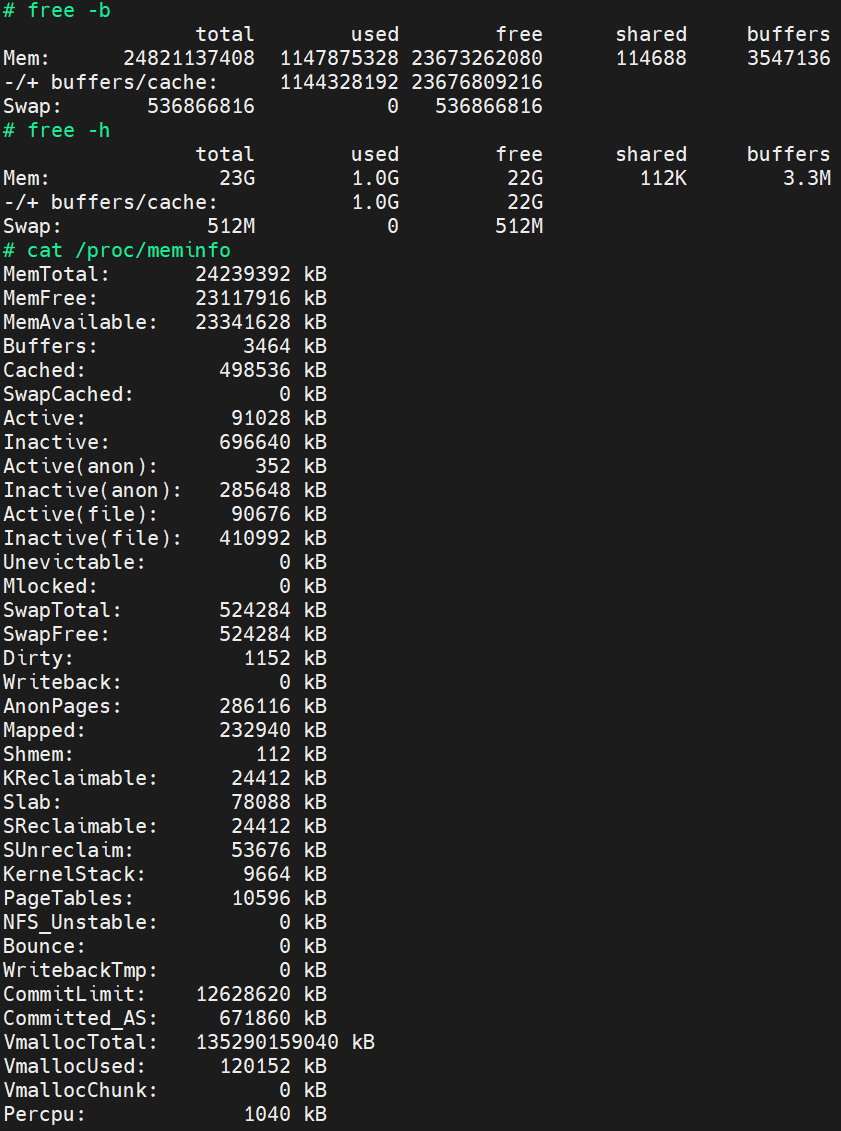
\includegraphics[width=0.8\textwidth]{mem.png}
  \caption{内存优化结果}
  \label{fig:memory}
\end{figure}

\subsection{启动时间验证（bootchart）}

使用 bootchart 工具采集系统启动过程的性能数据，具体步骤如下：

\textbf{Step 1：连接开发板并启用 bootchart}

\begin{lstlisting}[style=shell, caption={启用 bootchart}]
hdc shell
begetctl bootchart disable
begetctl bootchart enable
begetctl bootchart start
\end{lstlisting}

\textbf{Step 2：重启开发板开始采集}

\begin{lstlisting}[style=shell, caption={重启采集}]
reboot
# 重启完成后，再次进入 shell
hdc shell
\end{lstlisting}

\textbf{Step 3：停止采集并导出数据}

\begin{lstlisting}[style=shell, caption={停止采集并导出}]
begetctl bootchart stop

cd /data/service/el0/startup/init/
ls -l
# 会看到 4 个文件：header、proc_diskstats.log、proc_ps.log、proc_stat.log

# 打包数据
tar -czf bootchart.tgz *

exit
# 将文件导出到 PC
hdc file recv /data/service/el0/startup/init/bootchart.tgz ./
\end{lstlisting}

\textbf{Step 4：生成启动分析图表}

\begin{lstlisting}[style=shell, caption={生成启动分析图表}]
# 安装 bootchart 可视化工具
pip install pycairo-1.28.0-cp313-cp313-win_amd64.whl

# 解压bootchart-master，把拉取的 bootchart.tgz 文件放到 bootchart-master 目录下，并执行
python -m pybootchartgui.main .\bootchart.tgz
\end{lstlisting}
time
最后 bootchart-master 目录下可以读取到 bootchart.png

\begin{figure}[htbp]
  \centering
  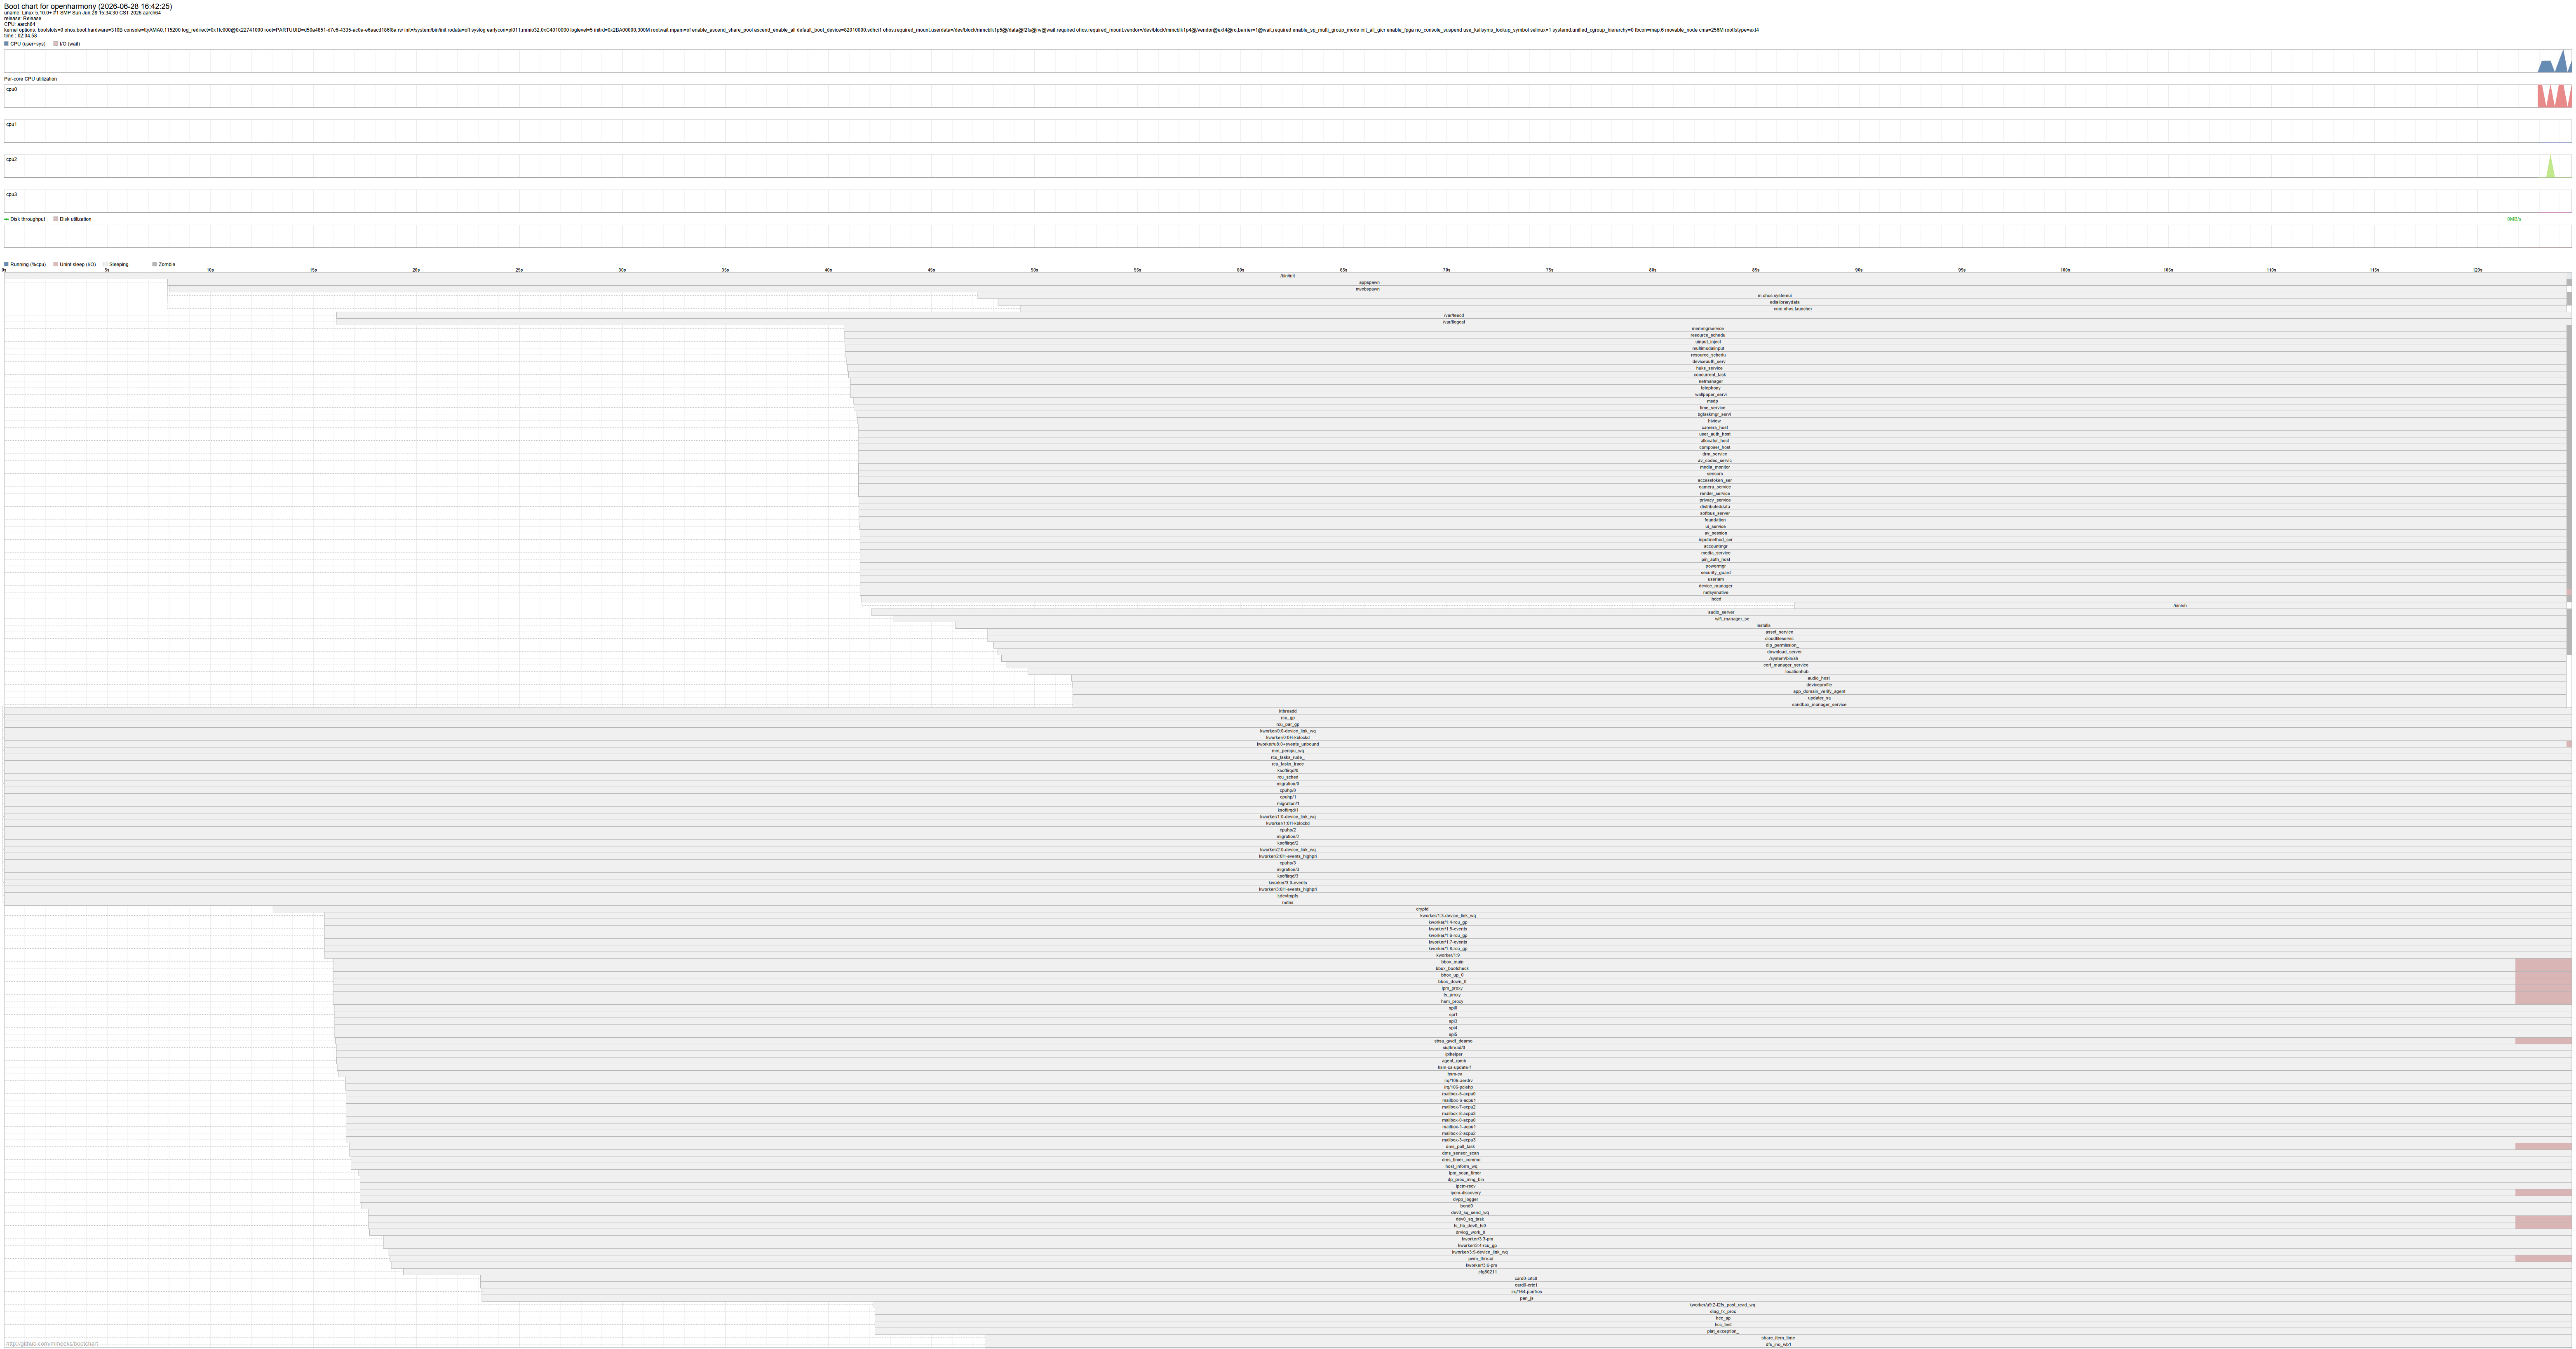
\includegraphics[width=0.8\textwidth]{bootchart.png}
  \caption{时间优化结果}
  \label{fig:time}
\end{figure}

\section{优化总结}

本章针对 OpenHarmony 系统在昇腾 310B 平台上的性能瓶颈，从内存和启动时间两个维度进行了系统性优化：

\begin{enumerate}
  \item \textbf{内存优化}：通过 MMZ 由 3072M 缩减到 1536M、ZRAM/VM 调优、NAPI 预加载由 81 项缩减到 26 项、预装应用缩减到 11 项及 46 项非必要 SA 停止自启动，首轮实测已将启动初始内存从 1.7GB 降至约 0.9GB，V1.11 在该基础上完成第二轮裁剪
  \item \textbf{启动时间优化}：通过移除未使用模块与网络初始化、删除固定等待、将延迟服务收敛到 3 个以及前移 CANN 服务依赖初始化，首轮启动时间已从 50s 缩短至约 42s，V1.11 完成单应用启动路径收敛
  \item \textbf{功能保护}：裁剪过程中明确保留显示、触摸、相机、HDMI 音频、媒体播放、HDC、CANN/NPU、本机 5001 推理服务及应用运行所需权限和资源，避免以破坏主业务换取指标
\end{enumerate}
